%%%
 % File:     spoofing.tex
 % Author:   Hackademics Forum <hackademicsforum6@gmail.com>
 % Project:  MindMap des vulnérabilités
 % Released: 03/08/2016
%%%

%!TeX root = main.tex
%!TeX encoding = UTF-8
%!TeX program = pdflatex
%!TeX spellcheck = fr_FR

%%%
 % Vulnérabilités Spoofing
%%%
\newpage
\section{Usurpation (Spoofing)}\label{vulnerabilites:reseau:spoofing}

Le spoofing est une vulnérabilité qui touche les plus importants protocoles réseau : IP, ARP, MAC, DNS.
Son utilisation permet à un attaquant de se faire passer pour ce qu'il n'est pas, %
afin de cacher ses actions ou de contourner des mécanismes de sécurité.

\subsection{IP Spoofing}\label{vulnerabilites:reseau:spoofing:ip}

Comme son nom l'indique l'IP Spoofing va se situer au niveau du protocole IP. L'attaque consiste à fabriquer et émettre vers une cible des paquets IP avec une fausse adresse d'origine. Cela va avoir deux conséquences :

\begin{itemize}
\item La cible va envoyer un ou des paquets de réponse à la machine dont l'adresse IP a été spoofée.
\item Si la cible utilise l'adresse IP d'origine pour filtrer les accès, elle va accepter des paquets IP qu'elle aurait dû refuser.
\end{itemize}

\begin{tabbing}
\end{tabbing}
L'IP Spoofing permet les types d'attaques suivants :

\begin{itemize}
\item Déni de service
\item Prise de controle
\end{itemize}

\subsubsection{Déni de service}\label{vulnerabilites:reseau:spoofing:ip:dos}

Actuellement le type d'attaque par IP Spoofing le plus utilisé est le déni de service distribué (en anglais DDOS / Distributed Denial Of Service). C'est le cas d'utilisation d'IP Spoofing le plus simple :
\begin{itemize}
\item L'attaquant va envoyer des quantités énormes de paquets IP vers des destinations diverses, en indiquant comme adresse IP d'origine l'adresse de la cible qu'il veut saturer.
\item Les destinataires des paquets vont renvoyer des réponses vers l'adresse qu'ils croient à l'origine.
\item Si le nombre de paquets réponses est suffisamment important, la cible, ou l'infra-structure qui l'héberge voit sa bande passante ou sa capacité de traitement saturée, ce qui rend ses services injoignables pour les utilisations légitimes.
\end{itemize}

\begin{figure}[hbtp]
\caption{Déni de service}
\centering
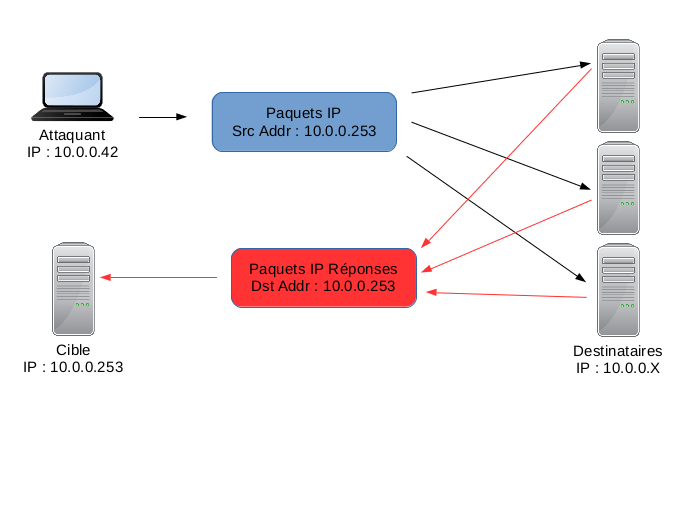
\includegraphics[scale=1]{../images/ip-spoofing-ddos.png}
\end{figure}

\begin{tabbing}
\end{tabbing}
Il existe divers outils pour créer de tels paquets IP. nmap est un des plus connus. Dans cet exemple, l'attaquant pourrait exécuter une commande semblable à :
\begin{center}
nmap -S 10.0.0.253 -e wlan0 -Pn 10.0.0.0/24
\end{center}


\subsubsection{Prise de controle}\label{vulnerabilites:reseau:spoofing:ip:control}

Certains types de services utilisent l'adresse IP des clients pour controler les accès. C'est le cas notamment des services rsh ou rlogin, qui servent à prendre à distance le controle d'un serveur. Ce type d'attaque tend à être de moins en moins utilisable, les services peu sécurisés comme rlogin et rsh n'étant quasimment plus utilisés.


Contrairement à l'attaque précédente, qui était relativement simple, celle-ci va être plus complexe à mettre en oeuvre. Elle nécessite en effet de connaître la ou les adresses IP autorisée(s) par la cible, et elle ne peut pas être exécutée en aveugle. Il faudra donc la coupler avec d'autres attaques afin de détourner le trafic destiné à l'adresse IP usurpée.


Les différentes étapes de cette attaque seront donc :

\begin{itemize}
\item Trouver l'adresse IP autorisée par la cible
\item Mettre hors service la machine autorisée (par un DOS par exemple) pour l'empêcher de répondre aux paquets éventuellement envoyés par la cible.
\item Prédire les numéros de séquence TCP de la cible.
\item Lancer l'attaque : envoyer à la cible un paquet TCP avec le flag SYN, sur le service ciblé.
\item La cible va répondre avec un paquet SYN-ACK.
\item Répondre à la cible avec un paquet ACK et le bon numéro de séquence TCP.
\item La connexion TCP est alors établie.
\item Envoyer un paquet PSH (remontant les données directement à l'application) pour envoyer une commande au service (exemple : echo ++ >> /.rhosts).
\end{itemize}
\begin{tabbing}
\end{tabbing}

L'attaque peut donc se résumer ainsi (ici, la machine A est celle de l'attaquant, C la machine autorisée, A(C) indiquant que A spoofe l'adresse de C) :

\begin{figure}[hbtp]
\caption{Prise de controle}
\centering
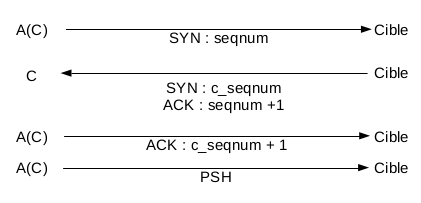
\includegraphics[scale=1]{../images/ip-spoofing-control.png}
\end{figure}

\subsubsection{Contre-mesures}\label{vulnerabilites:reseau:spoofing:ip:countermeasures}

Les contre-mesures contre l'IP Spoofing sont de plusieurs ordres. Certaines sont de la responsabilité des opérateurs internet, d'autres relèvent des sysadmin :

\begin{tabbing}
\end{tabbing}
\textbf{Opérateurs internet}

\begin{itemize}
\item Pour des attaques en aveugle, telles que celles utilisées par les DDOS en rebond, la balle est dans le camps des opérateurs : une adresse IP source peut en théorie etre bloquée au niveau d'un routeur BGP. Pour des raisons de performance, les opérateurs n'implémentent pas ce genre de controle.
\item Certains acteurs (opérateurs, hébergeurs, grands fournisseurs de services) proposent des solutions de mitigation des DDOS. Ces solutions consistent en gros à mobiliser une quantité de bande passante réseau suffisante pour absorber le trafic DDOS. Elles ont tendance à etre couteuses et ont parfois du mal à suivre la "course aux armements" face à des attaques de plus en plus importantes.
\end{itemize}

\begin{tabbing}
\end{tabbing}
\textbf{Sysadmin}
\begin{itemize}
\item Au niveau du réseau d'une organisation, meme très grande, ne pas se contenter de règles de filtrage par interfaces réseau, il faut y ajouter des filtres sur les adresses IP ou les sous-réseaux (subnets), appliquer une isolation stricte au niveau IP. Par exemple, une interface connectée au réseau 192.168.1.0/24 ne doit pas laisser passer de paquets venant d'une autre plage d'adresse.
\item Pour ce qui est de la prise de controle, la solution est plus simple : ne pas utiliser de services obsolètes comme rsh ou rlogin. Les services modernes de prise de controle à distance, comme SSH, sont une alternative adéquate. Le filtrage par IP peut rester nécessaire, par exemple pour l'accès à une interface de management web, mais ne doit pas être la seule protection. L'accès à ce genre d'UI devant être sécurisé par d'autres moyens (authentification SSL si possible par certificats).
\item La plupart des systèmes d'exploitation modernes rendent la prédiction des numéros de séquence TCP très difficile, voire quasimment impossible.
\item Il n'est pas certain que les objets connectés, de fonctionnalités minimales, appliquent les bonnes pratiques, tant au niveau système/réseau que controle d'accès. Des attaques record récentes (septembre 2016) ont utilisé massivement des caméras IP compromises, que les fournisseurs de solutions DDOS n'ont pas pu contrer (KrebsOnSecurity.com, par exemple).
\end{itemize}
\begin{tabbing}
\end{tabbing}



\subsection{ARP Spoofing}\label{vulnerabilites:reseau:spoofing:arp}

...

\subsection{MAC Spoofing}\label{vulnerabilites:reseau:spoofing:mac}

...

\subsection{DNS Spoofing}\label{vulnerabilites:reseau:spoofing:dns}

...

\endinput
